%% 
%% Copyright 2007-2020 Elsevier Ltd
%% 
%% This file is part of the 'Elsarticle Bundle'.
%% ---------------------------------------------
%% 
%% It may be distributed under the conditions of the LaTeX Project Public
%% License, either version 1.2 of this license or (at your option) any
%% later version.  The latest version of this license is in
%%    http://www.latex-project.org/lppl.txt
%% and version 1.2 or later is part of all distributions of LaTeX
%% version 1999/12/01 or later.
%% 
%% The list of all files belonging to the 'Elsarticle Bundle' is
%% given in the file `manifest.txt'.
%% 

%% Template article for Elsevier's document class `elsarticle'
%% with numbered style bibliographic references
%% SP 2008/03/01
%%
%% 
%%
%% $Id: elsarticle-template-num.tex 190 2020-11-23 11:12:32Z rishi $
%%
%%
\documentclass[preprint,12pt]{elsarticle}

%% Use the option review to obtain double line spacing
%% \documentclass[preprint,review,12pt]{elsarticle}

%% Use the options 1p,twocolumn; 3p; 3p,twocolumn; 5p; or 5p,twocolumn
%% for a journal layout:
%% \documentclass[final,1p,times]{elsarticle}
%% \documentclass[final,1p,times,twocolumn]{elsarticle}
%% \documentclass[final,3p,times]{elsarticle}
%% \documentclass[final,3p,times,twocolumn]{elsarticle}
%% \documentclass[final,5p,times]{elsarticle}
%% \documentclass[final,5p,times,twocolumn]{elsarticle}

%% For including figures, graphicx.sty has been loaded in
%% elsarticle.cls. If you prefer to use the old commands
%% please give \usepackage{epsfig}

%% The amssymb package provides various useful mathematical symbols
\usepackage{amssymb}
%% The amsthm package provides extended theorem environments
%%\usepackage{amsthm}

%% The lineno packages adds line numbers. Start line numbering with
%% \begin{linenumbers}, end it with \end{linenumbers}. Or switch it on
%% for the whole article with \linenumbers.
\usepackage{lineno}

%% Русский язык - закомментировать в финальной версии
\usepackage[russian]{babel}

%% advanced mathematics
\usepackage{amsmath}
\usepackage[ruled]{algorithm2e}
\usepackage{multirow}

\usepackage{hyperref}

\journal{Knowledge-Based Systems}

\begin{document}

\begin{frontmatter}

%% Title, authors and addresses

%% use the tnoteref command within \title for footnotes;
%% use the tnotetext command for theassociated footnote;
%% use the fnref command within \author or \address for footnotes;
%% use the fntext command for theassociated footnote;
%% use the corref command within \author for corresponding author footnotes;
%% use the cortext command for theassociated footnote;
%% use the ead command for the email address,
%% and the form \ead[url] for the home page:
%% \title{Title\tnoteref{label1}}
%% \tnotetext[label1]{}
%% \author{Name\corref{cor1}\fnref{label2}}
%% \ead{email address}
%% \ead[url]{home page}
%% \fntext[label2]{}
%% \cortext[cor1]{}
%% \affiliation{organization={},
%%             addressline={},
%%             city={},
%%             postcode={},
%%             state={},
%%             country={}}
%% \fntext[label3]{}

\title{On hyperparameter tuning through Lipschitz global optimization} % and dimensionality reduction}?
%% О настройке гиперпараметров с помощью липшицевой глобальной оптимизации

%% use optional labels to link authors explicitly to addresses:
%% \author[label1,label2]{}
%% \affiliation[label1]{organization={},
%%             addressline={},
%%             city={},
%%             postcode={},
%%             state={},
%%             country={}}
%%
%% \affiliation[label2]{organization={},
%%             addressline={},
%%             city={},
%%             postcode={},
%%             state={},
%%             country={}}

\author[UNN,ITMO]{Konstantin Barkalov}
\author[UNN,ITMO]{Denis Karchkov}
\author[UNN,ITMO]{Evgeny Kozinov}
\author[UNN,ITMO]{Ilya Lebedev}
\author[UNN,ITMO]{Denis Rodionov}
\author[UNN,ITMO]{Marina Usova}

\affiliation[UNN]{organization={Lobachevsky University},%Department and Organization
            addressline={Gagarin Av. 23}, 
            city={Nizhni Novgorod},
            postcode={603022}, 
            %state={},
            country={Russia}}
						
\affiliation[ITMO]{organization={ITMO University},%Department and Organization
            addressline={Lomonosova St. 9}, 
            city={St. Petersburg},
            postcode={191002}, 
            %state={},
            country={Russia}}


\begin{abstract}
%% Text of abstract

На качество работы методов машинного обучения существенное влияние оказывают их гиперпараметры, при этом оценка критерия качества является трудоемкой операцией. Поэтому актуальной является задача разработки ителлектуальных методов для выбора оптимальных значений гиперпараметров, которые требуют малого числа поисковых испытаний.
В этой статье мы предлагаем новый подход к настройке гиперпараметров, основанный на идеях Lipschitz global optimization. 
В рамках данного подхода решение задач с несколькими параметрами сводится к решению эквивалентных им одномерных задач. Соответствующая редукция основана на использовании space-filling curves (Peano curves). 
Указанные подходы реализованы в open-source фреймворке методов интеллектуальной оптимизации iOpt.
Для демонстрации преимуществ iOpt проведено его сравнение с известными фреймворками Optuna и HyperOpt при настройке гиперпараметров различных методов машинного обучения на представительном наборе датасетов. Результаты показывают, что методы Lipschitz global optimization обеспечивают сравнимые по качеству результаты за существенно меньшее время по сравнению с известными алгоритмами настройки гиперпараметров.

\end{abstract}

%%Graphical abstract
%\begin{graphicalabstract}
%\includegraphics{grabs}
%\end{graphicalabstract}

%%Research highlights
\begin{highlights}
\item Для настройки гиперпараметров разработан фреймворк методов липшицевой оптимизации
\item Для решения многомерных задач используется редукция размерности на оснвое кривых Пеано
\item Предложена схема сведения задач, часть параметров которых является категориальными, к одной задаче с непрерывными параметрами 
\item Разработанные методы (в отличие от известных методов настройки гиперпараметров) являются детерминированными, что обеспечивает стабильный результат при разных запусках алгоритмов
\end{highlights}

\begin{keyword}
%% keywords here, in the form: keyword \sep keyword
Lipschitz optimization \sep Multiextremal function \sep Hyperparameter tuning

%% PACS codes here, in the form: \PACS code \sep code

%% MSC codes here, in the form: \MSC code \sep code
%% or \MSC[2008] code \sep code (2000 is the default)

\end{keyword}

\end{frontmatter}

\linenumbers

%% main text
\section{Introduction}
\label{sec_intro}

В настоящее время сложные научно и/или промышленные задачи чаще всего решаются численными методами. В большинстве таких методов, например, в методах машинного обучения, имеются гиперпараметры, от выбора конкретных значений которых может зависеть эффективность (в заданной метрике) полученного решения при заданных тем или иным способом ограничениях на время расчетов \cite{Hutter2019,nikitin2021}. Тот факт, что во многих случаях разница в эффективности получаемого решения при разных значениях гиперпараметров может быть достаточно значительной, привел к возникновению the hyperparameter optimization (HPO) problem, а также исследованиям подходов к ее решению, реализуемых в фреймворках автоматического подбора гиперпараметров \cite{Tune, optuna, hyperopt,Sherpa}. С математической точки зрения HPO problem соответствует задаче глобальной оптимизации с фиксированными границах изменения гиперпараметров. В некоторых случаях часть гиперпараметров может быть категориальной, то есть принимать значения лишь из некоторого, обычно небольшого, числа вариантов, что приводит к необходимости использовать методы оптимизации, способные решать задачи с дискретными параметрами.

Для конечного пользователя, желающего провести настройку используемого метода, подобрав оптимальное сочетание гиперпараметров, выбор конкретного фреймворка определяется следующими факторами: 1) эффективность реализованных в фреймворке методов, позволяющих решить HPO problem того класса задач, которому принадлежит задача пользователя; 2) простота использования фреймворка с точки зрения описания/формирования задачи подбора оптимального сочетания гиперпараметров, организации процесса поиска оптимума, а также получения и анализа результатов. В настоящее время наиболее распространенным способом организации такого интерфейса является использование языка программирования Python, при этом сами фреймворки могут быть написаны, как на этом, так и на других языках.

В данной статье мы представляем фреймворк методов интеллектуальной оптимизации iOpt\footnote{\url{https://github.com/aimclub/iOpt/}}, ориентированный на решение задач выбора оптимальных значений гиперпараметров различных алгоритмов (включая методы машинного обучения и эвристической оптимизации). Статья построена следующим образом. В начале приведен обзор известных методов, используемых для настройки гиперпараметров. В section \ref{sec_lip} приведена математическая постановка задачи, описаны одходы к редукции многомерных задач к одномерным и решению задач с дискретными параметрами. В section \ref{sec_iOpt} описана алгоритмическая основа методов глобальной оптимизации, реализованных во фреймворке iOpt. В section \ref{sec_exp} даны результаты численных экспериментов, проведенных для сравнения эффективности фреймворка iOpt с другими известными фреймворками на модельных и прикладных задачах. В заключении приведены выводы и планы по развитию фреймворка.


\section{Related work}
\label{sec_rel}

Основная сложность при решении HPO problem состоит в том, что поиск оптимального сочетания гиперпараметров требует для каждого выбранного варианта их значений решения соответствующей исходной задачи, например, задачи машинного обучения, а значит, может быть довольно длительным по времени. Таким образом, любой подход к решению HPO problem будет ограничен в числе сочетаний гиперпараметров, которое метод глобальной оптимизации сможет проверить прежде, чем будет исчерпан доступный вычислительный ресурс. Конечно, в таких условиях сложно говорить о сходимости метода к глобальному оптимуму или о каких-то гарантиях его отыскания. Речь может идти только о возможности получения приемлемого (с точки зрения исследователя) решения. Дадим краткую характеристику ряда методов, которые используются для задач настройки гиперпараметров (в зависимости от свойств исходно задачи).

Самым простым способом поиска глобального оптимума является метод полного перебора (поиска по равномерной \cite{Bao2006} или случайной \cite{Bergstra2012} сетке). Выбрав число анализируемых вариантов по каждому из гиперпараметров, перебрав все получившиеся сочетания и взяв наилучшее из них в заданной метрике, мы получим оценку оптимума с определенной точностью \cite{Nevendra2022}. Метод полного перебора прост в реализации, обладает идеальным параллелизмом, но имеет существенный недостаток – экспоненциальный рост числа узлов сетки с ростом числа гиперпараметров. Таким образом, в качестве метода для решения HPO problem полный перебор может использоваться только в «простых» задачах, где малО как число гиперпараметров (один-два), так и время решения исходной задачи при каждом выбранном их сочетании.

Альтернативой полному перебору при увеличении числа гиперпараметров являются метаэвристические (генетические и аналогичные) алгоритмы \cite{Opara2019}. Данные алгоритмы широко применяются при отсутствии формульного описания исследуемой модели (модель вида «черный ящик»), что характерно для рассматриваемых HPO problems \cite{Zhou2021,Yang2022}. Метаэвристические алгоритмы слабо зависят от числа гиперпараметров, используют информацию с предыдущих итераций для выполнения текущей, однако в силу заложенной в методы случайности дают гарантию отыскания глобального оптимума только в вероятностном смысле.

Еще один подход к поиску глобального оптимума -- байесовская оптимизация, также применяемая для решения задач вида «черный ящик» \cite{Frazier2018,Archetti2019}. Фактически методы байесовской оптимизации строят стохастическую модель оптимизируемой функции. Модель итерационно обновляется на основе накапливаемой в процессе поиска оптимума информации, позволяя на каждой очередной итерации оценить наиболее вероятное положение глобального оптимума. Методы байесовской оптимизации обладают существенно более высокой эффективностью в сравнении с полным перебором, но, тем не менее, также подвержены влиянию «проклятия размерности», пусть и в меньшей степени.

В известных фреймворках по настройке гиперпараметров широко используется алгоритм Tree-Structured Parzen Estimator (TPE) \cite{hyperopt,NIPS2011}. TPE -- это итерационный алгоритм, идейно близкий к методам байесовской оптимизации. Перед началом работы алгоритма должна быть задана область поиска в пространстве гиперпараметров и определена оптимизируемая функция. В процессе своей работы метод проводит испытания в области поиска, после чего на их основе строит оценки распределения лучших и всех остальных результатов в пространстве гиперпараметров. Далее проводится поиск сочетания гиперпараметров, которое дает максимальное ожидаемое улучшение. These hyperparameters are then evaluated on the objective function. Описанный процесс повторяется до достижения заданного числа итераций или до тех пор, пока не будет достигнуто ограничение по времени.

Хорошие результаты, достигаемые методами байесовской оптимизации  \cite{Joy2020} и TPE \cite{Watanabe2022a,Watanabe2022b}, основаны на априорном предположении, что функция соответствует определенной стохастической модели, например, Gaussian process \cite{Rasmussen2005}. Однако в глобальной оптимизации существуют и иные предположения о виде функции, которые дают замечательные результаты.

Одним из таких допущений о решаемой задаче является предположение об ограниченности относительных изменений целевой функции. В этом случае говорят, что функция удовлетворяет условию Липшица, а решаемая задача называется задачей липшицевой глобальной оптимизации. Для класса задач липшицевой глобальной оптимизации разработан целый ряд эффективных алгоритмов \cite{Jones2021,Paulavicius2020,Strongin2020,Sergeyev2017,PaulaviciusZilinskas2014}, которые превосходят многие другие методы глобальной оптимизации \cite{Sergeyev2018} и показали свою применимость ряде приложений \cite{Kvasov2008,CANDELIERI2019,Gubaydullin2021}.
 
Фреймворк iOpt содержит реализацию алгоритмов липшицевой оптимизации, являющихся развитием информационно-статистического алгоритма глобального поиска, детально описанного в \cite{Strongin2000,Sergeyev2013}. 
В частности, методы были адаптированы для решения задач с частично целочисленными параметрами, которые весьма часто встречаются в задачах HPO.
Результаты экспериментов, приведенные в Section \ref{sec_exp}, показывают, что в задачах HPO фреймворк iOpt не уступает известным фреймворкам аналогичного назначения (таким как Optuna \cite{optuna} and HyperOpt \cite{hyperopt}).

\section{Lipschitz optimization} 
\label{sec_lip}

\subsection{Problem statement} 

Мы будем рассматривать задачу поиска глобального минимума в следующей постановке:
\begin{gather}
	\varphi(y^*) = \min \varphi(y), \; y \in D, \label{f_func} \\
	D = \left\{y \in R^N : a_j \leq y_j \leq b_j , \; 1 \leq j \leq N \right\}. \label{f_D}
\end{gather}

Будем также предполагать, что целевая функция $\varphi(y)$ удовлетворяет в области поиска $D$ условию Липшица, т.е.
\begin{equation} \label{f_lip}
	\left| \varphi(y')-\varphi(y'') \right| \leq L\left\| y' - y''  \right\| , \; y',y'' \in D, \; 0<L<\infty.
\end{equation}
Здесь $ \left\| \cdot \right\|$ обозначает евклидову норму, а константа $L$ является априори не известной и подлежит оценке в процессе решения. 
%Такие задачи называются задачами липшицевой глобальной оптимизации with box-constraints.

Функция $\varphi(y)$ предполагается многоэкстремальной и заданной в виде ``черного ящика'', т.е. некоторого алгоритма вычисления ее значений. Кроме того, подразумевается, что каждое поисковое испытание (т.е. вычисление значения функции в точке допустимой области) требует значительных вычислительных ресурсов. Такая постановка проблемы полностью соответствует задаче настройки гиперпараметров методов машинного обучения \cite{Joy2020,Wang2021}.

Условие Липшица допускает следующую геометрическую интерпретацию. Допустим, что одномерная липшицева функция $f(x)$ (с известной константой Липшица $L$) была вычислена в двух точках $x'$ и $x''$. В соответствии с условием (\ref{f_lip}) выполняются следующие неравенства, характеризующие поведение функции $f(x)$ на интервале $[x', x'']$:
\begin{gather*}
	f(x) \leq f(x') + L(x-x'), \; x \geq x',\\
	f(x) \geq f(x') - L(x-x'), \; x \geq x',\\
	f(x) \leq f(x') - L(x-x''), \; x \leq x'',\\
	f(x) \geq f(x') + L(x-x''), \; x \leq x''.
\end{gather*}

В силу данных неравенств значения функции в точках интервала $[x', x'']$ должны располагаться внутри области, ограниченной прямыми, проходящими через точки $(x', f(x'))$ и $(x'', f(x''))$ с наклоном $L$ и $-L$ (see Fig. \ref{fig1}).

\begin{figure}
\centering
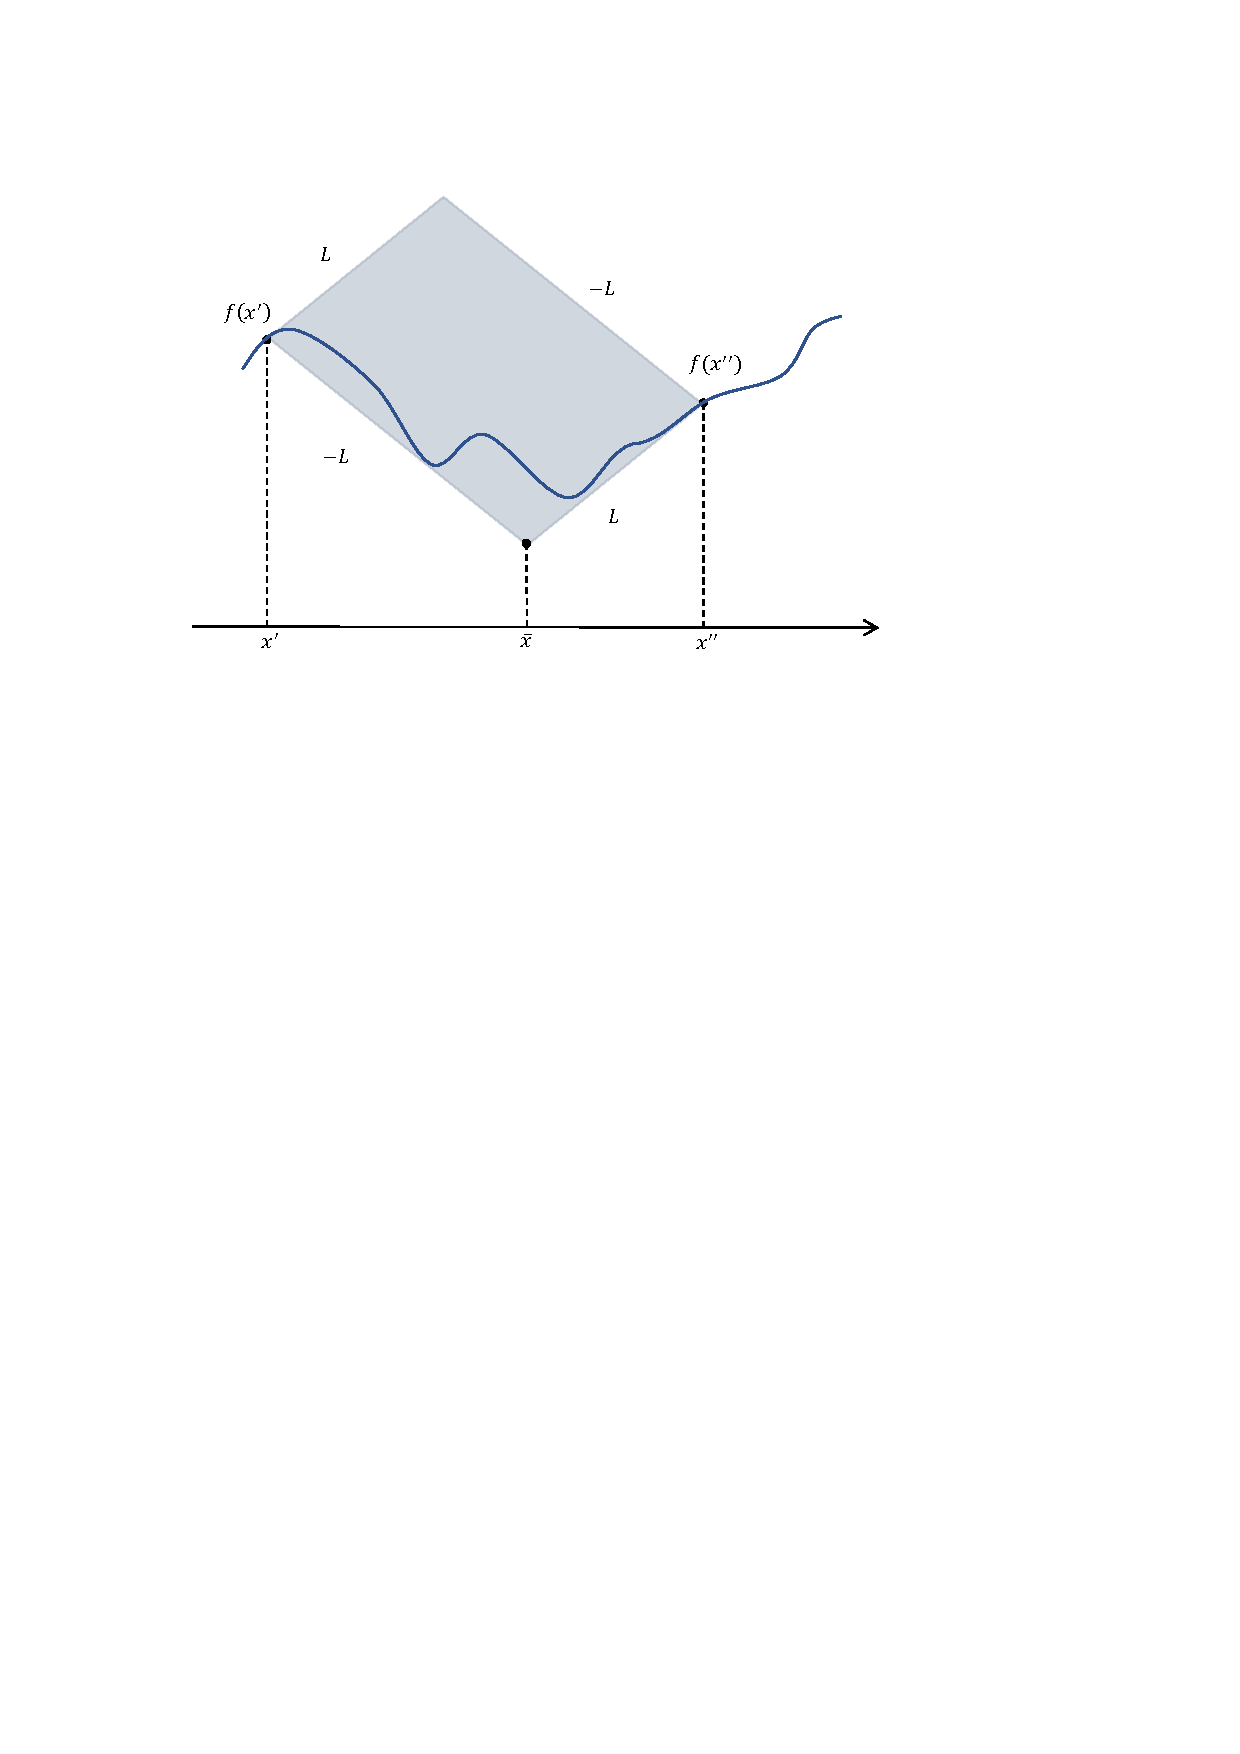
\includegraphics[width=0.8\textwidth]{Fig1.pdf}
\caption{Значения функции $f(x)$ должны находиться внутри области, выделенной цветом} \label{fig1}
\end{figure}


Также в соответствии с (\ref{f_lip}) может быть записано неравенство $f(x) \geq F(x)$, где функция $F(x)$ (называемая минорантой) определяется в соответствии с формулой
\[
F(x) = \max\left\{f(x') - L(x-x'),f(x') + L(x-x'')\right\}, \; x\in [x', x''].
\] 

Наименьшее значение миноранты $F(x)$ на $[x', x'']$ совпадает с оценкой наименьшего значения функции $f(x)$ на данном интервале. Указанная оценка достигается в точке 
\[
\overline{x} = \frac{x'+x''}{2}-\frac{f(x'')-f(x')}{2L}
\] 
и равна
\[
F(\overline{x}) = \frac{f(x')+f(x'')}{2} -L \frac{x''-x'}{2}.
\]

Методы липшицевой глобальной оптимизации используют эту идею в своих вычислительных правилах; на ней также основано и доказательство их сходимости (see, e.g.,
\cite{Jones2021,PaulaviciusZilinskas2014,Sergeyev2013,Evtushenko2013}).

\subsection{Проблема редукции размерности} 

Одной из основных трудностей при решении многомерных задач глобальной оптимизации является рост вычислительных затрат при увеличении размерности задачи. Эта сложность имеет место и при решении задач липшицевой глобальной оптимизации.
Например, решение задачи (\ref{f_func}) c помощью поиска по равномерной сетке с шагом $\epsilon$ потребует проведения 
\[
K \approx \prod_{j=1}^N{\frac{b_j-a_j}{\epsilon}}
\]
испытаний. Очевидно, что $K$ экспоненциально возрастает с ростом $N$.
Уменьшение числа испытаний при тех же требованиях к точности решения возможно за счет адаптивного построения неравномерной сетки в области изменения параметров.

Известным подходом к решению многомерной задачи (\ref{f_func}) является ее редукция к одномерной задаче с последующим применением эффективных одномерных алгоритмов глобальной оптимизации (see \cite{Strongin2000,Sergeyev2013}). Здесь хорошо зарекомендовал себя подход, в котором размерность задачи редуцируется при помощи кривой Пеано–Гильберта $y(x), x \in [0, 1]$.
Такая кривая однозначно и непрерывно отображает интервал $[0, 1]$ на гиперинтервал $D$ из (\ref{f_D}), т.е. заполняет всю область $D$.

Для решения задачи глобальной липшицевой оптимизации кривые, заполняющие пространство, могут быть применены следующим образом.
Если $y(x)$ есть кривая Пеано–Гильберта, то из непрерывности целевой функции $\varphi(y)$ следует, что
\[
\min_{y \in D } \varphi(y) = \min_{x \in [0,1] } \varphi(y(x)),
\]
т.е. исходная многомерная задача (\ref{f_func}) редуцируется к одномерной.


При этом известно (see \cite{Strongin2000}), что если многомерная функция $\varphi(y), \; y \in D,$  удовлетворяет условию Липшица с константой $L$, то редуцированная одномерная функция $\varphi(y(x)), \; \in [0,1]$ удовлетворяет the H{\"o}lder condition
\[
\left|\varphi(y(x'))-\varphi(y(x''))\right|\leq H\left|x'-x''\right|^{1/N}, \; x',x''\in[0,1].
\]
Здесь $N$ есть размерность исходной задачи, а коэффициент $ H=2 L \sqrt{N+3}$.

Замечание 1. Для редуцированной одномерной функции $\varphi(y(x))$  не будет выполняться условие Липшица. Однако многие одномерные алгоритмы липшицевой оптимизации
могут быть обобщены на случай минимизации гeльдеровых функций. Конкретный пример такого обобщения приведен в subsection \ref{sec_GSA}. 

\begin{figure}
\center
\begin{minipage}{0.45\linewidth}
\center{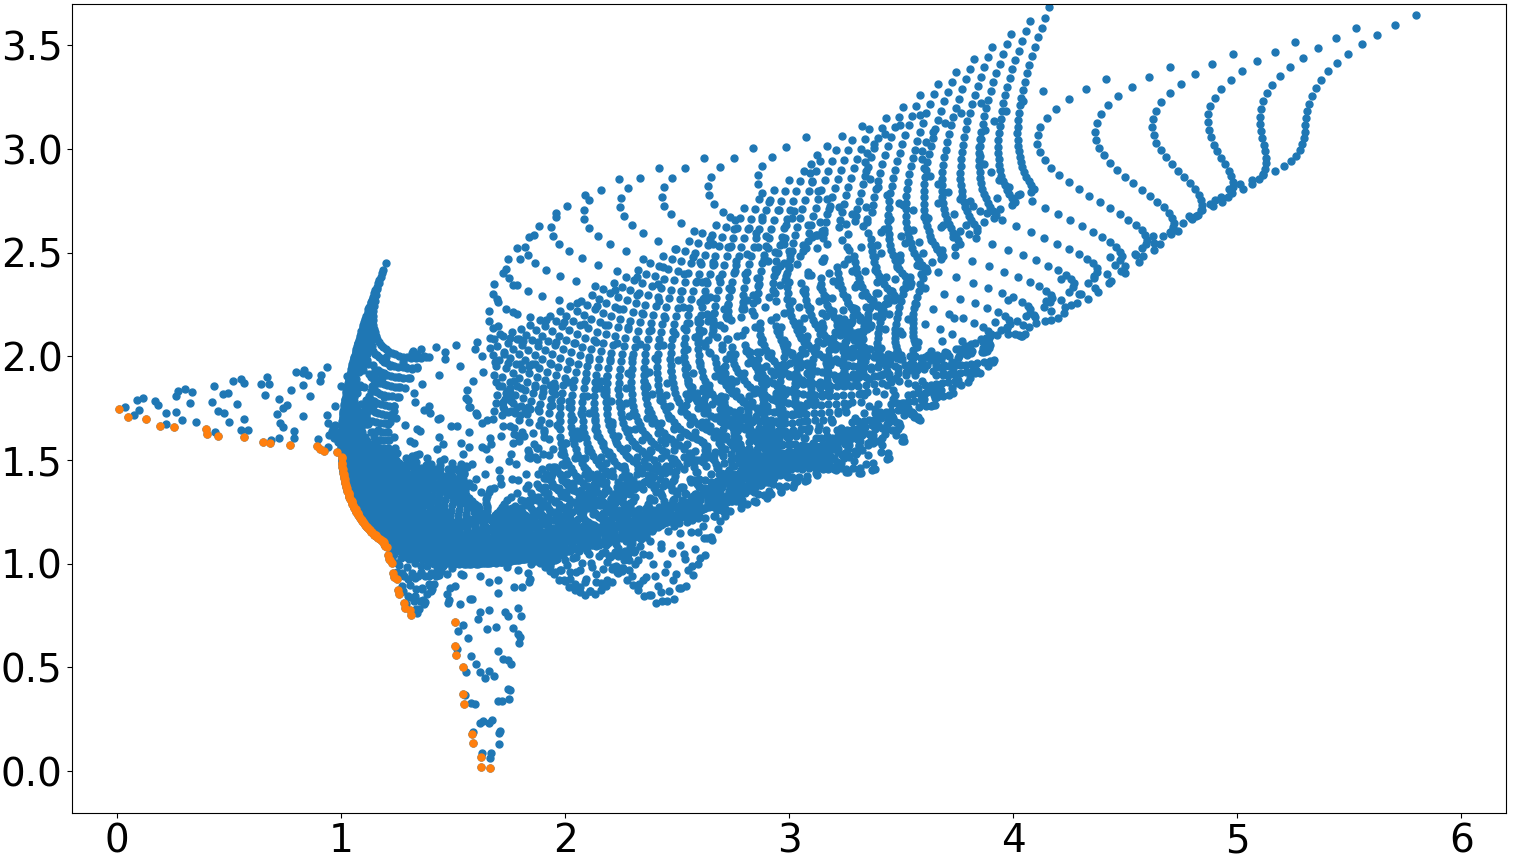
\includegraphics[width=0.9\linewidth]{fig2a.jpg} }
\end{minipage}
\begin{minipage}{0.45\linewidth}
\center{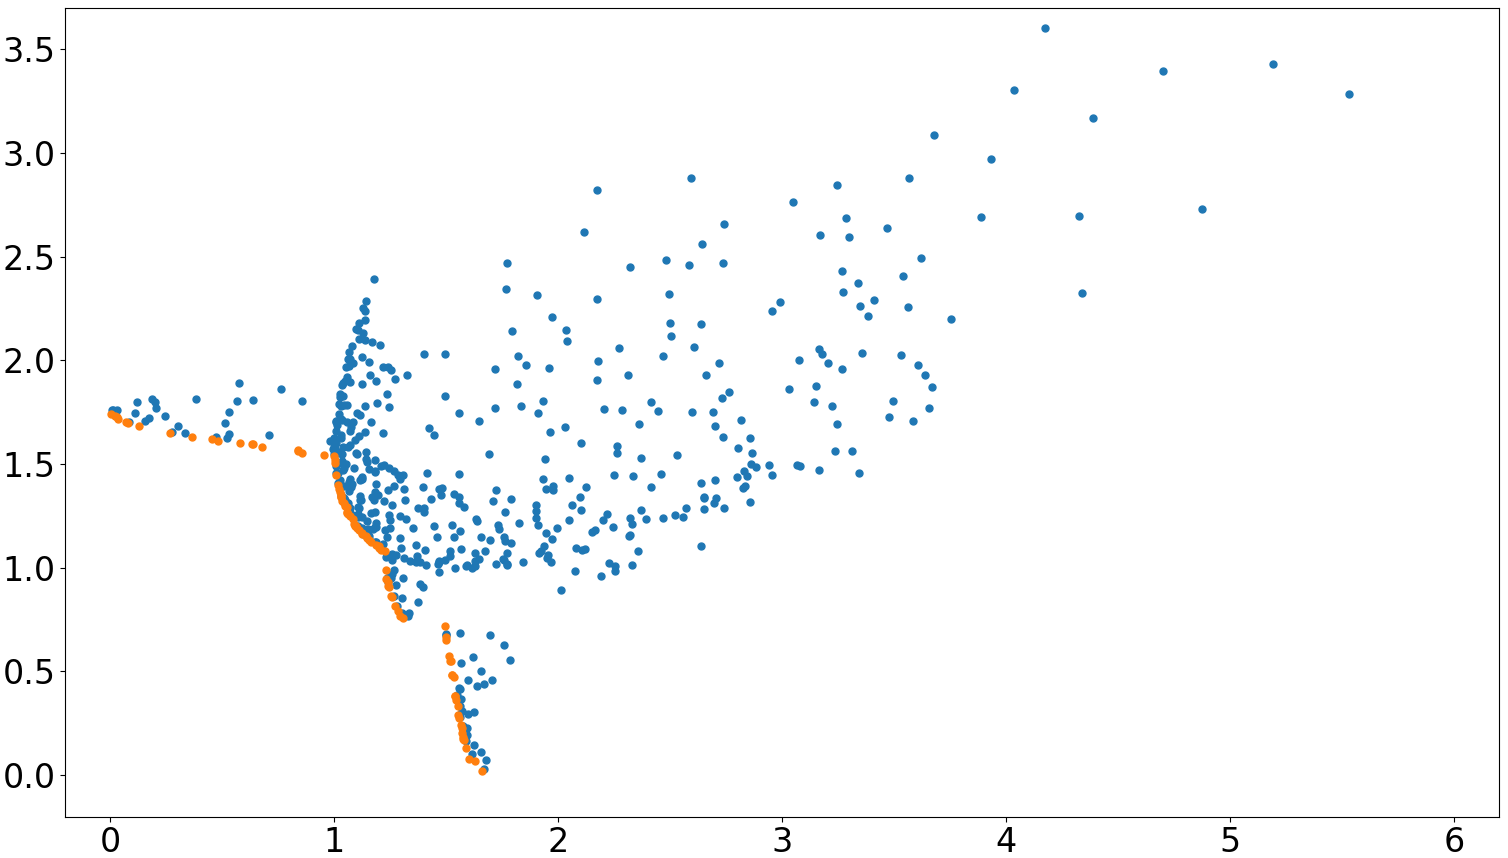
\includegraphics[width=0.9\linewidth]{fig2b.jpg} }
\end{minipage}
\caption{Evolvents $y_m(x)$ with $m=4$.}\label{fig:Peano}
\end{figure}   

Замечание 2. Теоретическая кривая Пеано-Гильберта $y(x)$ определяется как предельный объект. В численных алгоритмах применяются evolvents $y_m(x)$, аппроксимирующие истинную curve c заданным уровнем плотности $2^{-m}$, зависящим от требуемой точности поиска. Эффективные схемы вычисления нескольких видов evolvents подробно описаны в \cite{Sergeyev2013}.
Для иллюстрации на Fig.~\ref{fig:Peano} приведены графики, соответствующие разверткам $y_m(x)$ с плотностью $m=4$ для размерностей $N=2$ и $N=3$. 


\subsection{Проблема дискретных параметров}
\label{sec_discr} 

Особый интерес представляют задачи, в которых часть параметров может принимать значения из заранее заданного конечного множества, т.к. для них сложнее построить оценки оптимума по сравнению с задачами с непрерывными параметрами.
Методам решения задач со смешанными параметрами посвящено много публикаций (см., например, обзоры \cite{Burer2012,Boukouvala2016}). 
Известные детерминированные методы решения задач данного класса ориентированы на решение линейных или выпуклых задач \cite{Lee2012}.
Сложные многоэкстремальные задачи предлагается решать с помощью эвристических подходов \cite{Belotti2013}.

Нами был предложен и реализован новый детерминированный подход к решению задач со смешанными параметрами; приведем здесь его краткое описание. 
Пусть  целевая функция задачи зависит от двух векторов параметров: вектора $y$, принадлежащего гиперинтервалу $D$, и вектора $u$, имеющий конечный (и при этом не очень большой) набор возможных значений, т.е. 
\begin{gather}\label{problem_i}
\min{\left\{ \varphi(y,u) : y\in D \right\}},\\
D=\left\{a_j \leq y_j \leq b_j, \; 1\leq j \leq N \right\}.\nonumber
\end{gather}

Такие конечные наборы значений могут характеризовать множество возможных сочетаний категориальных гиперпараметров исследуемого алгоритма машинного обучения. 
Характерными примером является support vector machine, влияние на качество работы которого оказывают непрерывные параметр регуляризации $C$ и коэффициент ядра $\gamma$. При этом тип функции ядря выбирается из конечного множества вариантов (например, полиномиальная функция, радиальная базисная функция, сигмоид и т.д.).
%Целочисленные параметры = непрерывные параметры с округлением, добавить комментарий об этом?

Занумеруем целыми числами $s, 1\leq s \leq S,$ все различные комбинации категориальных параметров, т.е. сопоставим каждому номеру $s$ вектор $u_s$. 
Тогда рассматриваемая задача может быть записана в виде 
\begin{gather}\label{problem_is}
 \min_{s\in\{1,...,S\}}\left[\min{\left\{ \varphi(y,u_s) : y\in D \right\}}\right].
\end{gather}

Используя схему редукции размерности с помощью кривых Пеано $y(x), x\in [0,1]$ можно сопоставить каждой задаче минимизации по $y$ одномерную задачу минимизации
\[
 \min{\left\{ \varphi(y(x),u_s): x \in [0,1] \right\}}, s \in \{1,...,S\}.
\]

Рассмотрим теперь отображение 
\[
Y(x)=y(x-E(x)), \; x\in[0,S],
\]
переводящее любую точку интервала [0,S] на область $D$ (обозначение $E(x)$ соответствует целой части числа $x$) и определим функцию 
\[
f(x) = \varphi(Y(x),u_{E(x)+1}), x\in[0,S],
\]
имеющую, вообще говоря, разрывы в целочисленных точках $x_i = i, 1\leq i \leq S-1$.
Поэтому значения  $z_i = f(x_i)$ в этих точках будут считаться неопределенными и не будут использоваться в алгоритме.
%, а значения индекса -- равным 0, т.е. $\nu(x_i) = 0$.

Используя введенные обозначения можно переформулировать исходную задачу как
\begin{equation}\label{problem_is1}
\min \left\{f(x): x \in [0,S] \right\}.
\end{equation}

Применяя к решению задачи (\ref{problem_is1}) алгоритм глобального поиска, мы найдем решение задачи (\ref{problem_i}). При этом основная часть испытаний будет проведена в $s$-й подзадаче, решение которой соответствует решению исходной задачи (\ref{problem_i}). В остальных подзадачах будет проведена лишь незначительная часть испытаний, т.к. решения данных подзадач являются локально-оптимальными по отношению к решению $s$-й подзадачи.

\section{iOpt framework} 
\label{sec_iOpt}


Фреймворк методов интеллектуальной оптимизации iOpt разработан в рамках выполенния проекта ``Strong Artificial Intelligence in Industry''.
Он предназначен для выбора оптимальных (в заданной метрике) значений параметров сложных объектов и процессов, например, методов искусственного интеллекта и машинного обучения. Фреймворк позволяет проводить точную настройку параметров моделей и методов, используемых в прикладных исследованиях в различных научных областях. Фреймворк iOpt разработан на языке программирования Python с использованием его стандартной библиотеки. Для его использования необходим установленный интерпретатор языка Pyhon версии не ниже 3.8. Фреймворк является open source и доступен по адресу https://github.com/aimclub/iOpt.

Фреймворк iOpt может использоваться при создании специализированных систем поддержки принятия решений для решения задач выбора оптимальных параметров сложных моделей или методов. Область применения фреймворка фокусируется на задачах настройки гиперпараметров, поскольку при решении задач этого класса возникают проблемы многоэкстремальности критерия оптимизации и отсутствия формульного описания исследуемой модели (модель вида «черный ящик»). 


\subsection{Global search algorithm}
\label{sec_GSA}

Алгоримтическим ядром фреймворка iOpt является информационно-статистический алгоритм глобального поиска для решения задач вида (\ref{f_func}), (\ref{f_D}). 
Данный алгоритм предполагает построение последовательности точек $y^i$, в которых проводятся поисковые испытания, т.е. вычисляются значения objective function $z^i = \varphi(y^i)$. В соответствии с используемой схемой редукции размерности проведение испытания подразумевает вычисление $y^i=y(x^i))$, поэтому результатом испытания будет являться набор значений $(x^i, y^i=y(x^i), z^i = \varphi(y^i))$. 
Поисковую информацию, накопленную после проведения $k$ испытаний, удобно представлять в виде множества, в котором соответствующие наборы перенумерованы (нижним индексом) в порядке возрастания $x$, т.е. в виде множества 
\begin{equation}\label{omega}
\Omega_k = \left\{  (x_i, y_i=y(x_i), z_i = \varphi(y_i)): 1 \leq i \leq k  \right\},	
\end{equation}
где $x_1 < x_2 < ... < x_k$.



Основная идея алгоритма глобального поиска состоит в следующем.
Пусть в процессе поиска проведено $k \geq 2$ испытаний and the search information $\Omega_k$ from (\ref{omega}) is obtained.
Для выбора точки очередного испытания для каждого поискового интервала $(x_{i-1},x_i), 1<i\leq k$, вычисляется его характеристика в соответствии с формулой
\begin{equation}\label{R}
R(i) = \Delta_i + \frac{(z_i-z_{i-1})^2}{(r\mu)^2\Delta_i}-2\frac{z_{i-1}+z_i}{r\mu}.	
\end{equation}
Здесь $r>1$ -- параметр алгоритма, $\Delta_i=(x_i-x_{i-1})^{1/N}$. Значение $\mu$ является нижней оценкой константы Гельдера целевой функции, вычисленной на основе поисковой информации из (\ref{omega}) по формуле
\begin{equation}\label{mu}
\mu = \max_{1<i\leq k}\frac{\left|z_i-z_{i-1}\right|}{\Delta_i},
\end{equation}
причем в случае, если формула (\ref{mu}) выдает значение $\mu=0$, то используется значение $\mu=1$.

Новое испытание проводится в точке $x^{k+1}$, принадлежащей интервалу с наибольшей характеристикой. Если правая точка этого интервала имеет номер $t$ в множестве $\Omega_k$, то формула для вычисления $x^{k+1}$ будет выглядеть следующим образом:
\begin{equation}\label{xk1}
x^{k+1} = \frac{x_t+x_{t-1}}{2}- \frac{\mathrm{sign}(z_t-z_{t-1})}{2r} \left(\frac{\left|z_t-z_{t-1}\right|}{\mu}\right)^N.   
\end{equation}


Algorithm \ref{alg_GSA} shows the pseudo code of the Global Search Algorithm.
Входными данными алгоритма являются objective function $\varphi(y)$  и область поиска $D$ из (\ref{f_func}) and (\ref{f_D}), параметр алгоритма $r>1$, точность поиска минимума $\epsilon > 0$, максимально допустимое число испытаний $K_{max}$. Выходным параметром алгоритма является оценка точки глобального минимума $y_{min}$. Дополнительными выходными параметрами могут быть значение функции в точке минимума $\varphi(y_{min})$ и число проведенных испытаний $k$.

\begin{algorithm}
\LinesNumbered
 \KwIn{$\varphi(y), D, r, \epsilon, K_{max}$}
 \KwOut{$y_{min}$}
 Initialize $k=2$, $\Omega_k= \left\{ (x_1=0, y_1=y(x_1), z_1=\varphi(y_1)), (x_2=1, y_2=y(x_2), z_2=\varphi(y_2)) \right\}$\\
 \While{ $\Delta_t \geq \epsilon$ and  $k \leq K_{max}$}{
  Вычислить оценку H\"older constant $\mu$ в соответствии с (\ref{mu})\\
	\For{$i=1$ \KwTo $k$}{
	Вычислить характеристику $R(i)$ в соответствии с (\ref{R})\\
	}
	Определить номер $t$, для которого $R(t) = \max \left\{ R(i), 1 \leq i \leq k \right\}$
	
	Вычислить точку нового испытания $x^{k+1}$ в соответствии с (\ref{xk1})
	
	Провести новое испытание в точке $x^{k+1}$
	
	Добавить $(x^{k+1}, y^{k+1}, z^{k+1})$ в множество $\Omega_k$
	
  $k = k + 1$\\
 }
 $l = \arg \min \left\{ z_i, 1 < i \leq k \right\}$\\
 $y_{min} = y_l$, \\ 
 \KwRet{$y_{min}$}
 \caption{Global search}\label{alg_GSA}
\end{algorithm}

Теория сходимости алгоритма, а также некоторые его модификации представлены в \cite{Strongin2000}.

\subsection{GSA for the problems with categorical parameters}
\label{sec_mGSA}

Рассмотрим случай, когда в настраиваемом алгоритме имеются как непрерывные, так и категориальные параметрами. 
В этом случае категориальным параметрам можно поставить в соответствие целочисленные значения, и свести сзадачу к постановке (\ref{problem_is1}).
Так как решение задач с частично целочисленными параметрами в соответсвии со схемой, изложенной в Section \ref{sec_discr}, предполагает решение задачи (\ref{problem_is1}) с разрывной целевой функцией, требуется модификация алгоритма, учитывающая эту особенность.

С этой целью введем классификацию точек из области поиска с помощью специального индекса $\nu_i=\nu(x_i)$.
Индексы целочисленных точек $x_i = i, 0\leq i \leq S$, будем полагать равным нулю, т.е. $\nu(x_i) = 0$. Для всех остальных значений $x\in(i,i+1),  0 \leq i < S$, значение индекса будем считать равным единице, т.е. $\nu(x) = 1$. Тогда результатом испытания в некоторой точке $x^j\in[0,S]$ будет являться набор значений
$(x^j, \nu^j=\nu(x^j), y^j=y(x^j), z^j = \varphi(y^j))$. Причем в случае $\nu^j=0$ значение $z^j$ будет считаться неопределенным.

Общая вычислительная схема, изложенная в виде Алгоритма \ref{alg_GSA}, останется прежней. Модификации будут состоять в следующем.
Модификации будут состоять в следующем.

1. На этапе инициализации в множество $\Omega_k$, содержащее поисковую информацию, заносятся значения $(x^i = i, \nu^i=0, y^i=y(x^i), z^i)$, $ i, 0\leq i \leq S$, т.е. заносятся граничные точки интервалов $(x_{i-1},x_i), 1<i\leq S$.
После этого проводятся испытания в произвольных внутренних точках (например, в серединах) интервалов $(x_{i-1},x_i), 1<i\leq S$; результаты испытаний также добавляются в поисковую информацию. 
Таким образом, после инициализации множество $\Omega_k$ будет содержать $k=2S+1$ элемент.

2. Вычисление оценки константы Гельдера $\mu$ в соответствии с формулой (\ref{mu}) должно выполняться только для  интервалов, для которых $\nu(x_i) = \nu(x_{i-1}) = 1$, т.е. когда значения $z_i$ and $z_{i-1}$ определены.

3. Вычисление характеристики поискового интервала $(x_{i-1},x_i), 1<i\leq k$, проводится по следующим правилам:
\begin{gather}\label{R_int}
R(i) = \Delta_i + \frac{(z_i-z_{i-1})^2}{(r\mu)^2\Delta_i}-2\frac{z_{i-1}+z_i}{r\mu}, \; \mathrm{if} \; \nu(x_i) = \nu(x_{i-1}) = 1, \nonumber \\ 
R(i) = 2\Delta_i-4\frac{z_i}{r\mu}, \; \mathrm{if} \;  \nu(x_i) = 1, \nu(x_{i-1}) = 0, \nonumber \\ 
R(i) = 2\Delta_i-4\frac{z_{i-1}}{r\mu}, \; \mathrm{if} \;  \nu(x_{i-1}) = 1, \nu(x_{i}) = 0. \nonumber
\end{gather}
Отметим, что в процессе работы алгоритма не будет возникать интервалов, у которых обе граничные точки имеют неопределенные значения функции, т.е. $\nu(x_i) = \nu(x_{i-1}) = 0$.

4. Точка нового испытания $x^{k+1}$ будет вычисляться следующим образом:
\begin{gather}\label{xk1_int}
x^{k+1} = \frac{x_t+x_{t-1}}{2}- \frac{\mathrm{sign}(z_t-z_{t-1})}{2r} \left(\frac{\left|z_t-z_{t-1}\right|}{\mu}\right)^N, \; \mathrm{if} \; \nu(x_i) = \nu(x_{i-1}) = 1, \nonumber \\    
x^{k+1} = \frac{x_t+x_{t-1}}{2} , \; \mathrm{if} \; \nu(x_i) \neq \nu(x_{i-1}). \nonumber
\end{gather}
Здесь $t$ есть номер поискового интервала, имеющего максимальную характеристику.

Еще раз отметим, что характеристика $R(i)$ количественно оценивает возможность нахождения точки $x^*$, являющейся inverse image of the global optimizer $y* = y(x^*)$, в пределах рассматриваемого интервала $(x_{i-1},x_i)$.

\section{Numerical experiments}
\label{sec_exp}

\subsection{Experimental setup}

Datasets

\begin{table}[]
\caption{14 datasets used in the experiments.}
\label{tab:1}
\begin{tabular}{lllllll}
\hline
Name                                                            & Num   & Attributes & Int & Float & Categorical & Classes \\ \hline
Balance                                                         & 625   & 4          & 4   & 0     & 0           & 3       \\
Bank Marketing                                                  & 45211 & 20         & 6   & 4     & 10          & 2       \\
Banknote                                                        & 1372  & 4          & 0   & 4     & 0           & 2       \\
Breast Cancer                                                   & 569   & 9          & 9   & 0     & 0           & 2       \\
CarEvaluation                                                   & 1728  & 6          & 0   & 0     & 6           & 4       \\
CNAE9                                                           & 1080  & 856        & 856 & 0     & 0           & 9       \\
Credit Approval                                                 & 690   & 15         & 0   & 6     & 9           & 2       \\
Digits                                                          & 5620  & 64         & 64  & 0     & 0           & 10      \\
Ecoli                                                           & 336   & 7          & 0   & 7     & 0           & 8       \\
Parkinsons                                                      & 197   & 22         & 0   & 22    & 0           & 2       \\
Semeion                                                         & 1593  & 256        & 256 & 0     & 0           & 10      \\
\begin{tabular}[c]{@{}l@{}}Statlog \\ Segmentation\end{tabular} & 2310  & 19         & 1   & 18    & 0           & 7       \\
Wilt                                                            & 4889  & 5          & 0   & 5     & 0           & 2       \\
Zoo                                                             & 101   & 16         & 16  & 0     & 0           & 7       \\ \hline
\end{tabular}
\end{table}

Metrics


% Please add the following required packages to your document preamble:
% \usepackage{multirow}
\begin{table}[]
\caption{Настраиваемые гиперпараметры для алгоритмов машинного обучения}
\label{tab:2}
\begin{tabular}{llll}
\hline
Метод                    & Параметры            & Тип параметра & Диапазон параметра                                                     \\ \hline
\multirow{7}{*}{XGBoost} & n\_estimators        & Int           & {[}10, 200{]}                                                          \\
                         & max\_depth           & Int           & {[}5, 20{]}                                                            \\
                         & min\_child\_weight   & Int           & {[}1, 10{]}                                                            \\
                         & Gamma                & Float         & {[}0.01, 0.6{]}                                                        \\
                         & Subsample            & Float         & {[}0.05, 0.95{]}                                                       \\
                         & colsample\_bytree    & Float         & {[}0.05, 0.95{]}                                                       \\
                         & learning\_rate       & Float         & {[}0.001, 0.1{]}                                                       \\ \hline
\multirow{3}{*}{\begin{tabular}[c]{@{}l@{}}Support \\ Vector   \\ Classification \\ (SVC)\end{tabular}} &
  Gamma &
  Float &
  {[}$10^{-9}$, $10^{-6}${]} \\
                         & C                    & Int           & {[}$10^1$,$10^{10}${]}                     \\
                         & Kernel               & Categorial    & \begin{tabular}[c]{@{}l@{}}\{‘poly’, ‘rbf’,\\ ‘sigmoid’\}\end{tabular} \\ \hline
\multirow{4}{*}{\begin{tabular}[c]{@{}l@{}}Multi-layer   \\ Perceptron \\ (MLP)\end{tabular}} &
  Activation &
  Categorial &
  \begin{tabular}[c]{@{}l@{}}\{'identity', \\ 'logistic', \\ 'tanh', 'relu'\}\end{tabular} \\
                         & hidden\_layer\_sizes & Int           & {[}2, 30{]}                                                            \\
                         & max\_iter            & Int           & {[}100, 700{]}                                                         \\
                         & Solver               & Categorial    & \begin{tabular}[c]{@{}l@{}}\{'lbfgs', 'sgd', \\ 'adam'\}\end{tabular}  \\ \hline
\end{tabular}
\end{table}

Algorithms for comparison

\subsection{Experimental results}

First result

Second result 

Third result


\begin{table}[]
\caption{Время поиска значений гиперпараметров при однократном запуске алгоритма оптимизации.}
\label{tab:3}
\begin{tabular}{lllllll}
\hline
Dataset &
  \begin{tabular}[c]{@{}l@{}}Optuna \\ random\end{tabular} &
  \begin{tabular}[c]{@{}l@{}}Optuna \\ tpe\end{tabular} &
  \begin{tabular}[c]{@{}l@{}}Optuna \\ cmaes\end{tabular} &
  \begin{tabular}[c]{@{}l@{}}Optuna \\ nsgaii\end{tabular} &
  \begin{tabular}[c]{@{}l@{}}Hyperopt\\ tpe\end{tabular} &
  iOpt \\ \hline
Balance                                                         & 10.8   & 9.2    & 9.0    & 10.6   & 10.3   & \textbf{7.7}    \\
\begin{tabular}[c]{@{}l@{}}Bank \\ Marketing\end{tabular}       & 2888.5 & 3406.5 & \textbf{2704.7} & 3078.6 & 3190.3 & 2963.3 \\
Banknote                                                        & 31.9   & \textbf{12.0}   & 17.7   & 22.1   & 21.7   & 18.4   \\
\begin{tabular}[c]{@{}l@{}}Breast \\ Cancer\end{tabular}        & 9.3    & 7.6    & 6.3    & 8.1    & 8.5    & \textbf{6.0}    \\
CarEvaluation                                                   & 50.9   & 63.3   & 51.0   & 53.1   & 69.5   & \textbf{45.2}   \\
CNAE9                                                           & 295.6  & 207.6  & 318.4  & 262.2  & 253.5  & \textbf{144.9}  \\
\begin{tabular}[c]{@{}l@{}}Credit \\ Approval\end{tabular}      & 14.2   & 12.6   & 13.4   & 13.4   & 15.8   & \textbf{10.8}   \\
Digits                                                          & 132.8  & \textbf{57.5}   & 82.1   & 111.6  & 92.4   & 62.5   \\
Ecoli                                                           & 5.5    & 6.3    & 4.0    & 5.4    & 6.4    & \textbf{3.6}    \\
Parkinsons                                                      & 3.5    & 5.0    & 3.6    & 3.8    & 4.4    & \textbf{2.9}    \\
Semeion                                                         & 218.4  & 119.5  & 157.9  & 135.7  & 193.6  & \textbf{114.2}  \\
\begin{tabular}[c]{@{}l@{}}Statlog \\ Segmentation\end{tabular} & 156.1  & \textbf{55.4}   & 87.1   & 159.2  & 91.6   & 66.5   \\
Wilt                                                            & 70.0   & 75.8   & 68.5   & 67.4   & 78.2   & \textbf{60.9}   \\
Zoo                                                             & 3.0    & 3.9    & 3.0    & 3.1    & 4.2    & \textbf{1.8}    \\ \hline
\end{tabular}
\end{table}


\section*{CRediT authorship contribution statement}

\textbf{Konstantin Barkalov:} Supervision, Conceptualization, Writing - original draft.
\textbf{Denis Karchkov:} Software, Data curation.
\textbf{Evgeny Kozinov:} Methodology, Validation, Writing - original draft.
\textbf{Ilya Lebedev:} Software, Investigation, Writing - original draft.
\textbf{Denis Rodionov:} Software, Investigation.
\textbf{Marina Usova:} Visualization.


\section*{Declaration of competing interest}

The authors declare that they have no known competing financial interests or personal relationships that could have appeared to influence the work reported in this paper.

\section*{Code availability}
%проверить перевод
Software that implements all of the described methods is available in the open repository \url{https://github.com/aimclub/iOpt/}.

\section*{Acknowledgements}
%уточнить ссылку
This research was supported by the research center ``Strong Artificial Intelligence in Industry'' of ITMO University.



%% The Appendices part is started with the command \appendix;
%% appendix sections are then done as normal sections
%% \appendix

%% \section{}
%% \label{}

%% If you have bibdatabase file and want bibtex to generate the
%% bibitems, please use
%%
\bibliographystyle{elsarticle-num} 
\bibliography{bibliography}

%% else use the following coding to input the bibitems directly in the
%% TeX file.

%\begin{thebibliography}{00}

%% \bibitem{label}
%% Text of bibliographic item

%\bibitem{}

%\end{thebibliography}
\end{document}
\endinput
%%
%% End of file `elsarticle-template-num.tex'.
